\documentclass[usenames, dvipsnames]{article}      % article class
\usepackage[utf8]{inputenc}
\newcommand{\mytitle}{Hybrid tropical cyclone hazard modelling
%, focusing on storm surges on the US East coast
}
\newcommand{\penname}{Simon~Thomas}
\usepackage{moreverb}
\RequirePackage{fancyhdr}    % use fancyhdr to customize hdrs & ftrs
\RequirePackage[margin=2.5cm, headheight=15pt, includeheadfoot]{geometry}
\renewcommand{\headrulewidth}{0pt}   % suppress rule across top(fancyhdr default)
\setlength\headheight{26pt} %% just to make a warning go away.
\rhead{\thepage}  % right head page number.
% page number on right head
\lfoot{\penname}  % left foot author.
\cfoot{}
\rfoot{}
\pagestyle{fancy}  % use fancyhdr style

\usepackage{Theme/mystyle}
\usepackage{Theme/linkcolors}
\usepackage{Theme/referencing}
\usepackage{Theme/globals}
\graphicspath{{images/}{../images/}}
\addbibresource{references/generic_references.bib}
\addbibresource{references/references.bib}
\addbibresource{references/fluid_dynamics.bib}
\addbibresource{references/machine_learning.bib}
\addbibresource{references/global_warming.bib}
\addbibresource{references/programming.bib}
\addbibresource{references/surge.bib}
\addbibresource{references/tebbutt.bib}
\addbibresource{references/taleb.bib}
\addbibresource{references/evt.bib}
\addbibresource{references/cyclone.bib}
\addbibresource{references/meteorology.bib}

\addbibresource{phd.bib}
\renewcommand{\familydefault}{\sfdefault}

% \RequirePackage{fancyhdr}    % use fancyhdr to customize hdrs & ftrs
\RequirePackage[margin=2.5cm, headheight=15pt, includeheadfoot]{geometry}
\renewcommand{\headrulewidth}{0pt}   % suppress rule across top(fancyhdr default)
\setlength\headheight{26pt} %% just to make a warning go away.
\rhead{\thepage}  % right head page number.
% page number on right head
\lfoot{\penname}  % left foot author.
\cfoot{}
\rfoot{}
\pagestyle{fancy}  % use fancyhdr style

\RequirePackage[linesnumbered,ruled,vlined]{algorithm2e}

\usepackage{array}
\newcolumntype{L}[1]{>{\raggedright\let\newline\\\arraybackslash\hspace{0pt}}m{#1}}

\title{\vspace*{-100pt}\textbf{\mytitle}\vspace{-15pt}}
\date{\vspace{-10pt}\today \vspace{-15pt}}
\author{A Proposal for a PhD project 
at the AI4ER CDT program  \\
\penname 
}

\usepackage[fontsize=12pt]{fontsize}
\begin{document}
\maketitle

\vspace{-10pt}\vspace{-5pt}

\footnotesize{
This proposal is the result of my own work and includes nothing which is the outcome of work done in collaboration, except where specifically indicated in the text and/or bibliography.}

\vspace{-10pt}

\normalsize

\subsection*{\vspace{-10pt}Motivation}


Tropical cyclones (TCs) have been the
largest physical hazard for economic 
damage~\cite{Chavas2013U.S.Perspective, shultz2005epidemiology},
and TC storm surges is the largest for lives
lost~\cite{shultz2005epidemiology, emanuel2005divine,
Rappaport2014FatalitiesInterpretation, zhang2009tropical}.
This hazard is increasing as more people live on vulnerable 
coastlines in substandard buildings~\cite{emanuel2005divine}.
Climate change is expected to exacerbate this,
as it begins to increase the maximum TC intensity\footnote{
However the uptick in TCs is not currently above
natural variability~\cite{mendelsohn2012impact}.}~\cite{
emanuel2008hurricanes,emanuel2017will, nordhaus2010} and
range~\cite{emanuel2008hurricanes, emanuel2017will, fedorov2010tropical}.
Sea level rise will also place 
more areas at risk~\cite{SROCC}.

Storm surges are coastal sea levels which
far exceed those expected given the tide.
They are caused by TCs and extratropical cyclones (ECs).
TCs draw their kinetic energy from the thermodynamic
disequilibrium between the tropical sea surface and the
troposphere~\cite{emanuel1986air, emanuel1987dependence}.
\iffalse
TCs are able to sustain very low central
pressures\footnote{As low as 870 hPa~\cite{Hoarau2017DidPressure}}
and azimuthal velocities, which create dangerous
surges~\cite{emanuel2005divine}.
\fi

It is necessary to quantify how this hazard will
change so that the public can act with foresight.
Others have already applied machine learning (ML) techniques to
this end~\cite{kulp2019new, kulp2018coastaldem, tadesse2020data}.
The motivation for hybrid physical/ML modelling is simple:
an algorithm that does not respect physical laws may fit
the data well, but it is more likely to generalise
poorly to unseen data~\cite{beucler2019achieving}. 
In general, observational data is highly correlated, 
extremes are necessarily rare, and so efficient use
must be made of the existing information.\vspace{-5pt}

\subsection*{Initial direction (9-12 months) -- hybrid extreme value theory 
            and the emulation of storm surge models}

\vspace{-10pt}
Chavas et al.~2013~\cite{Chavas2013U.S.Perspective} (C13)
demonstrated that using physical covariates such as
the maximum windspeed of the TC on landing,
and the mean slope to the 30m isobath improved the ability
of the extreme value theory (EVT) model~\cite{coles2001introduction}
to fit the hazard data over the East US coastline.
However, it did not systematically test whether
other physical measures might be more informative.
For example, the central pressure of the storm is generally
a more informative indicator of the hazard of a TC than the windspeed~\cite{Chavas2017PhysicalRelationship}.

 My MSci project\footnote{
 Full MSci report: \url{https://bit.ly/msci-report}; 
 Summary MSci report: \url{https://bit.ly/msci-summary}
 .} 
 showed that you can predict the
 responsiveness of a coastline to a wind stress fairly well with a
 simple physical model in Figure~\ref{fig:responsiveness}.
 This metric captured the broad trends seen in the model output.
 Therefore, given that this and other metrics could contain more
 information than the slope to the 30m isobath, I propose that we
 initially replicate and expand upon C13 with attempts to show whether
 additional metrics would be useful.\footnote{This idea was initially
 proposed by Dr.~Dan Chavas (Purdue), who was keen to see if his work could be
 improved upon. If the work goes as planned, it should lead to a publication before the 1st year report.}

\begin{figure}[htb!]
    \centering
    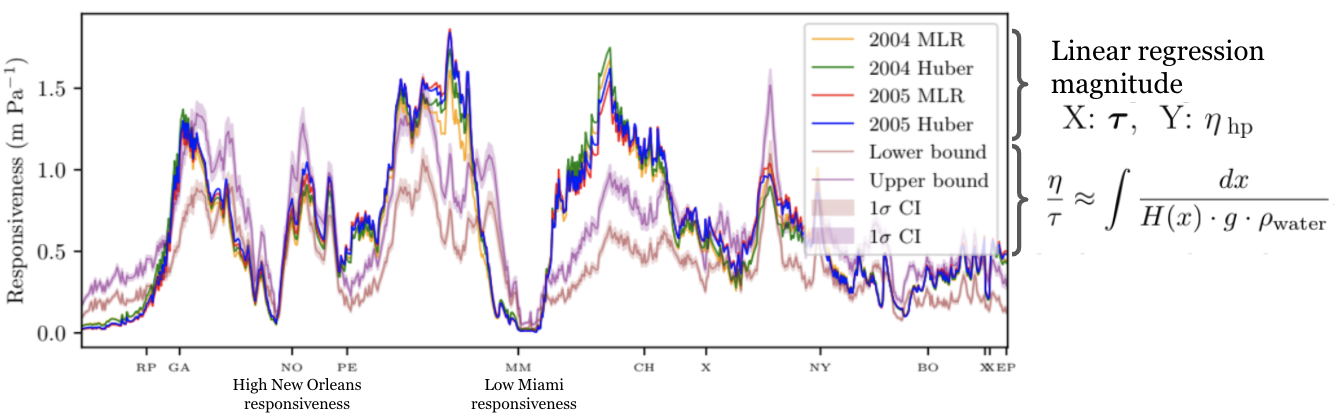
\includegraphics[width=1.1\linewidth]{img.png}
    \caption{The simple responsiveness metric from my MSci thesis. 
        A comparison between the calculated linear responsiveness
        of an hourly ORCA12 model to a wind stress, 
        and a na\"ive theoretical prediction based on 
        the bathymetry assuming a steady state box model.}
        \vspace{-10pt}
    \label{fig:responsiveness}
\end{figure}

This metric was developed 
in response to trying to analyse and explain the 
characteristics of physical model output with known theory.
Therefore, future progress is likely also dependent 
on more physical and statistical experimentation.
Prof.~Talea Mayo (Emory University) has offered to provide
an initial storm surge dataset that was produced in
collaboration with Prof.~Ning Lin (Princeton) with high resolution simulations 
of historical storm surges~\cite{Marsooli2019ClimatePatterns, Marsooli2018NumericalCoasts, Lin2015GreyCyclones}. 
The initial scientific questions to address would be:
\begin{itemize}
\addtolength\itemsep{-3mm}
\iffalse
    \item Is it possible to build a statistical or machine 
        learning type model with a variety of features 
        (e.g.~bathymetry, local winds) to better predict
        storm surge risk?
    
    \item Are there metrics that can summarise the bathymetry’s
        effect on the size of the storm surge from a given 
        tropical cyclone?
    \item Can we extend this framework to other forms
        of risk (e.g.~wind damage)?
\fi
\iftrue
    \item Is it possible to build extreme value theory model
        with a variety of physical covariates 
        (measures of e.g.~bathymetry, central pressure)
        to better predict storm surge risk after C13? 
        Can this be extended to other forms of risk?
        
    \item Can we use extreme value theory, constrained by our physical
        understanding of tropical cyclones, to describe long-term risks 
        (see Appendix~\ref{sec:frechet})?
        
\fi

    \item Are there effective methods of 
        emulating the high resolution storm 
        surge model~\cite{Ma2020MultifidelitySurge} 
        using e.g.~a convolutional neural
        network~\cite{Ronneberger2015U-Net:Segmentation,
        beucler2019achieving, beucler2019achieving} 
        and a cheaper physical 
        models~\cite{Akbar2013HybridModeling}.
        
        \vspace{-10pt}
\end{itemize}

\subsection*{\vspace{-5pt} Subsequent trajectory (18-20 months) -- hybrid surge downscaling}

Acquiring real knowledge about the future hazards of climate change
from climate models requires that we use robust methods to go from
model scale (a few kilometres resolution at best) to the real observed
surge. At the same time we need to try to account for the 
large scale model biases (e.g.~\cite{seager2019strengthening}).
This is known as downscaling, and is normally reliant on 
complicated statistical models (statisitical
downscaling)~\cite{Sithara2021StatisticalApproaches}
or high resolution physical models (dynamical
downscaling)~\cite{Barnard2019DynamicChange, Muis2020AProjections,
Dieterich2019ExtremeSensitivity, Troselj2021DynamicalJapan}.
A combination of the two (hybrid downscaling) has also been
used~\cite{Erlandsen2020AChange, Huang2014DownscalingApproach}.


Building a hybrid model to downscale from climate models 
to real extreme values is a much more significant task.
To begin with ECMWF/ORAS4 reanalyses
products~\cite{Zuo2019TheAssessment,Zuo2017TheSignals, OceanECMWF}
could be used as the input, and the results 
could be compared against the abundant
tide gauge data off the US East Coast~\cite{CO-OPSCurrents}.
The initial methods would be inspired and adapted 
from the models which were best able to emulate storm surge models in the 
first year.\footnote{This could be linked to the EnvSensors project~\cite{EnvironmentalInstitute}, where Dan Jones is a PI.}
This work could be progressively generalised to test if it works with 
different reanalyses products, and for example to any instrumented regions
of the East Asian coastline (see Appendix~\ref{sec:pub} for a breakdown by 
plausible publication).

If this model is reliable it could be used on the the CMIP6 ensemble
to calculate what the probable change in hazard along the East US coastline 
is over the next few decades (e.g.~\cite{Rahmstorf2017RisingFlooding}).


\printbibliography

\appendix

% \section{Examples of using Extreme Value Theory}



\section{Argument for the unphysicality of Frech\'et fits}
\label{sec:frechet}

\begin{figure}
    \centering
    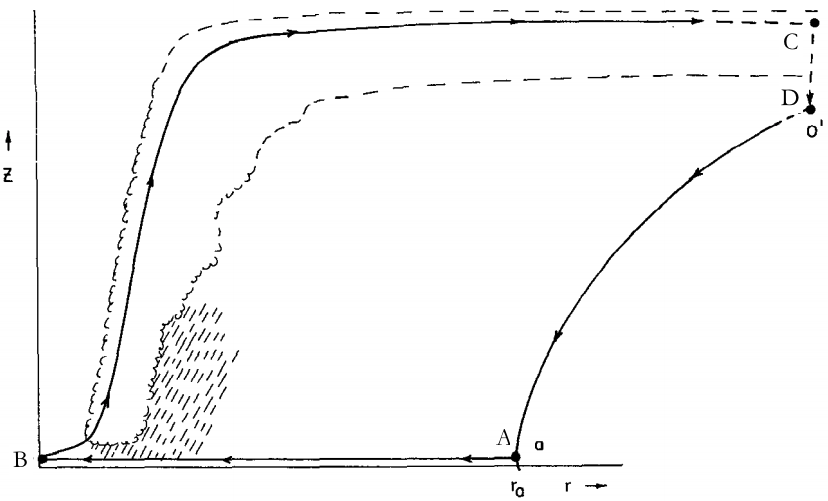
\includegraphics[width=0.45\linewidth]{hurricane-carnot.png}
    % \hpad
    %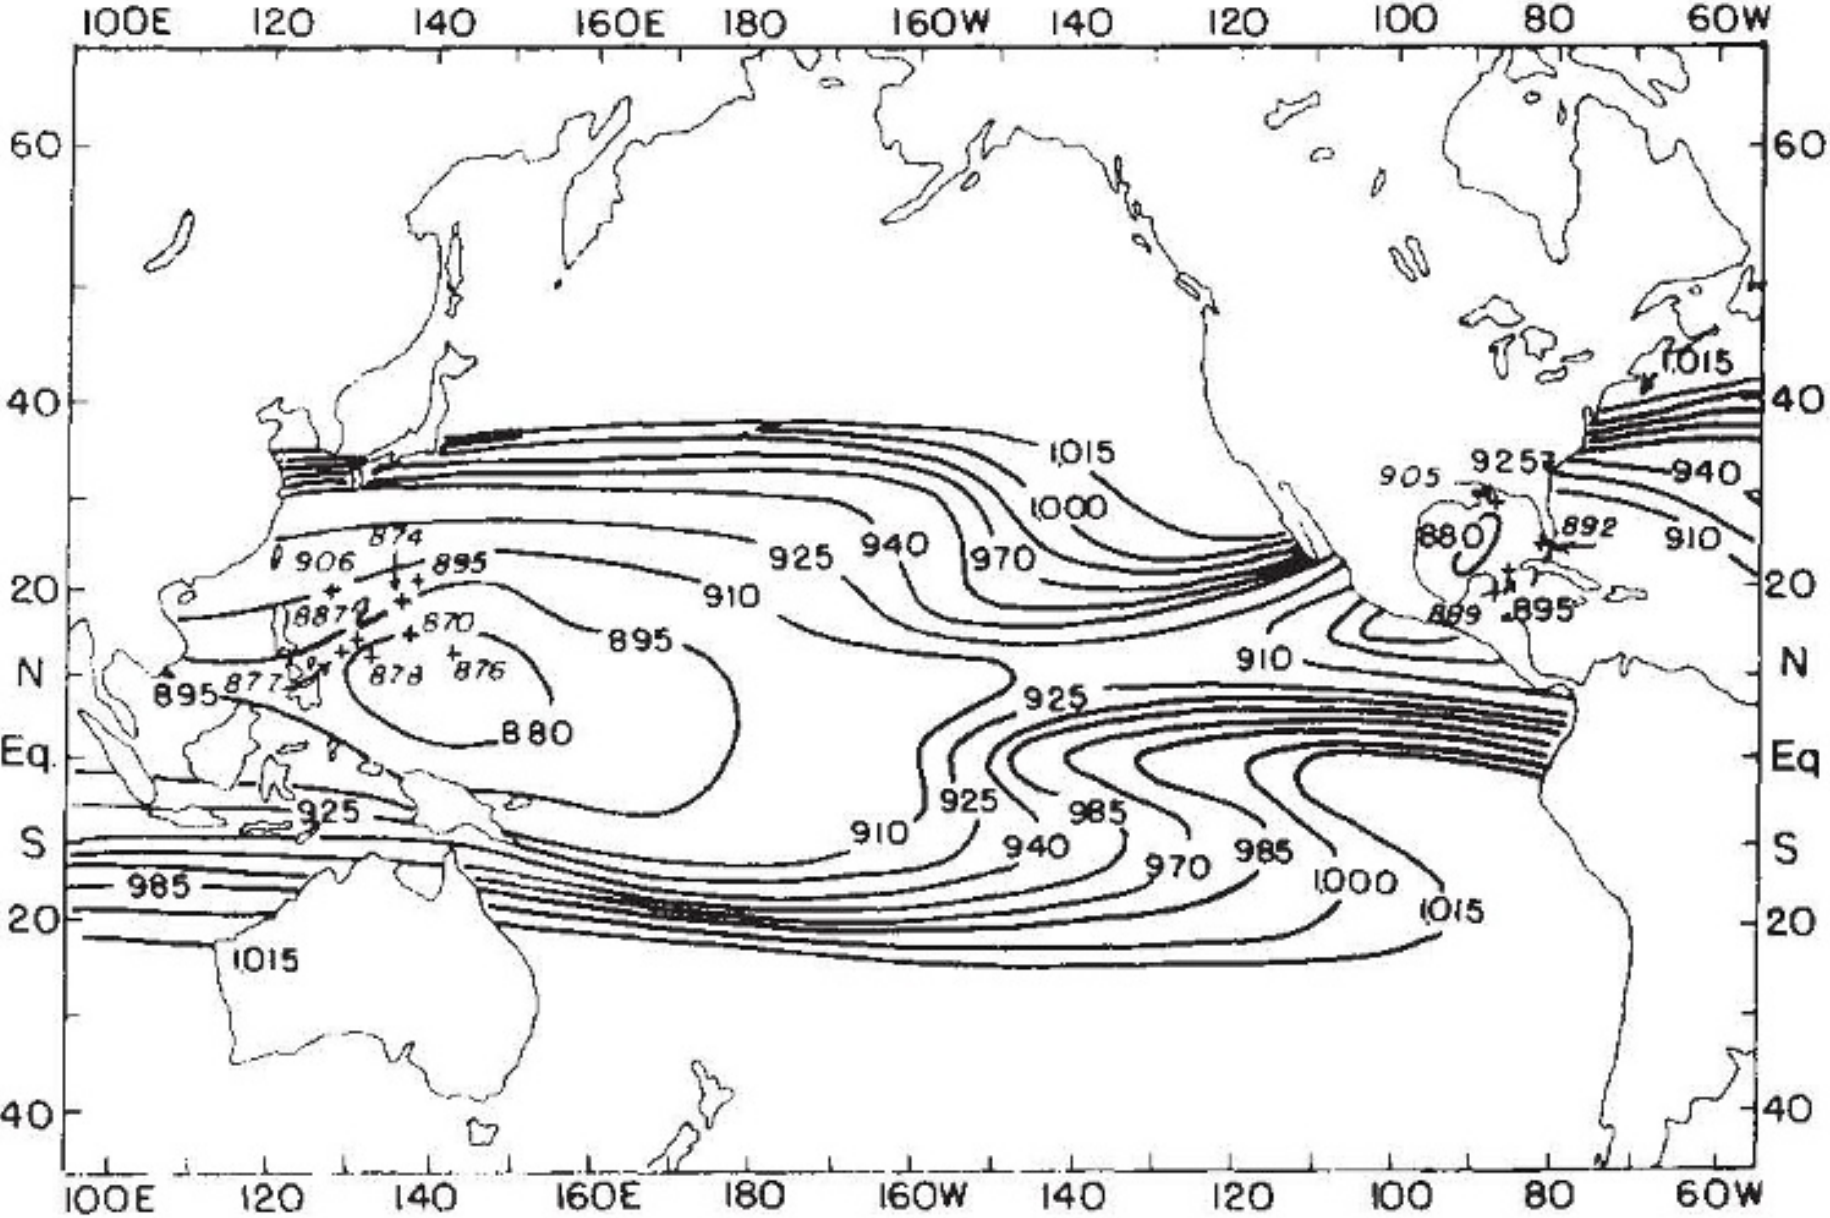
\includegraphics[width=0.45\linewidth]{e87-slimmed-verif.png}
    \caption{An explanation of the potential intensity
            from~\cite{emanuel1987dependence}.
            The figure shows the Carnot engine, that takes
            in heat energy as it goes across the sea surface (isotherm),
            goes up an adiabat along the eye wall and 
            out to the edge of the storm.
            Loses heat as it descends (isotherm), and
            then is pulled back into the storm (adiabat).
            The work from the heat engine then drives the surface
            waves, sea surface gradient, and upwelling of colder
            waters from the thermocline.
    }
    \label{fig:carnot}
    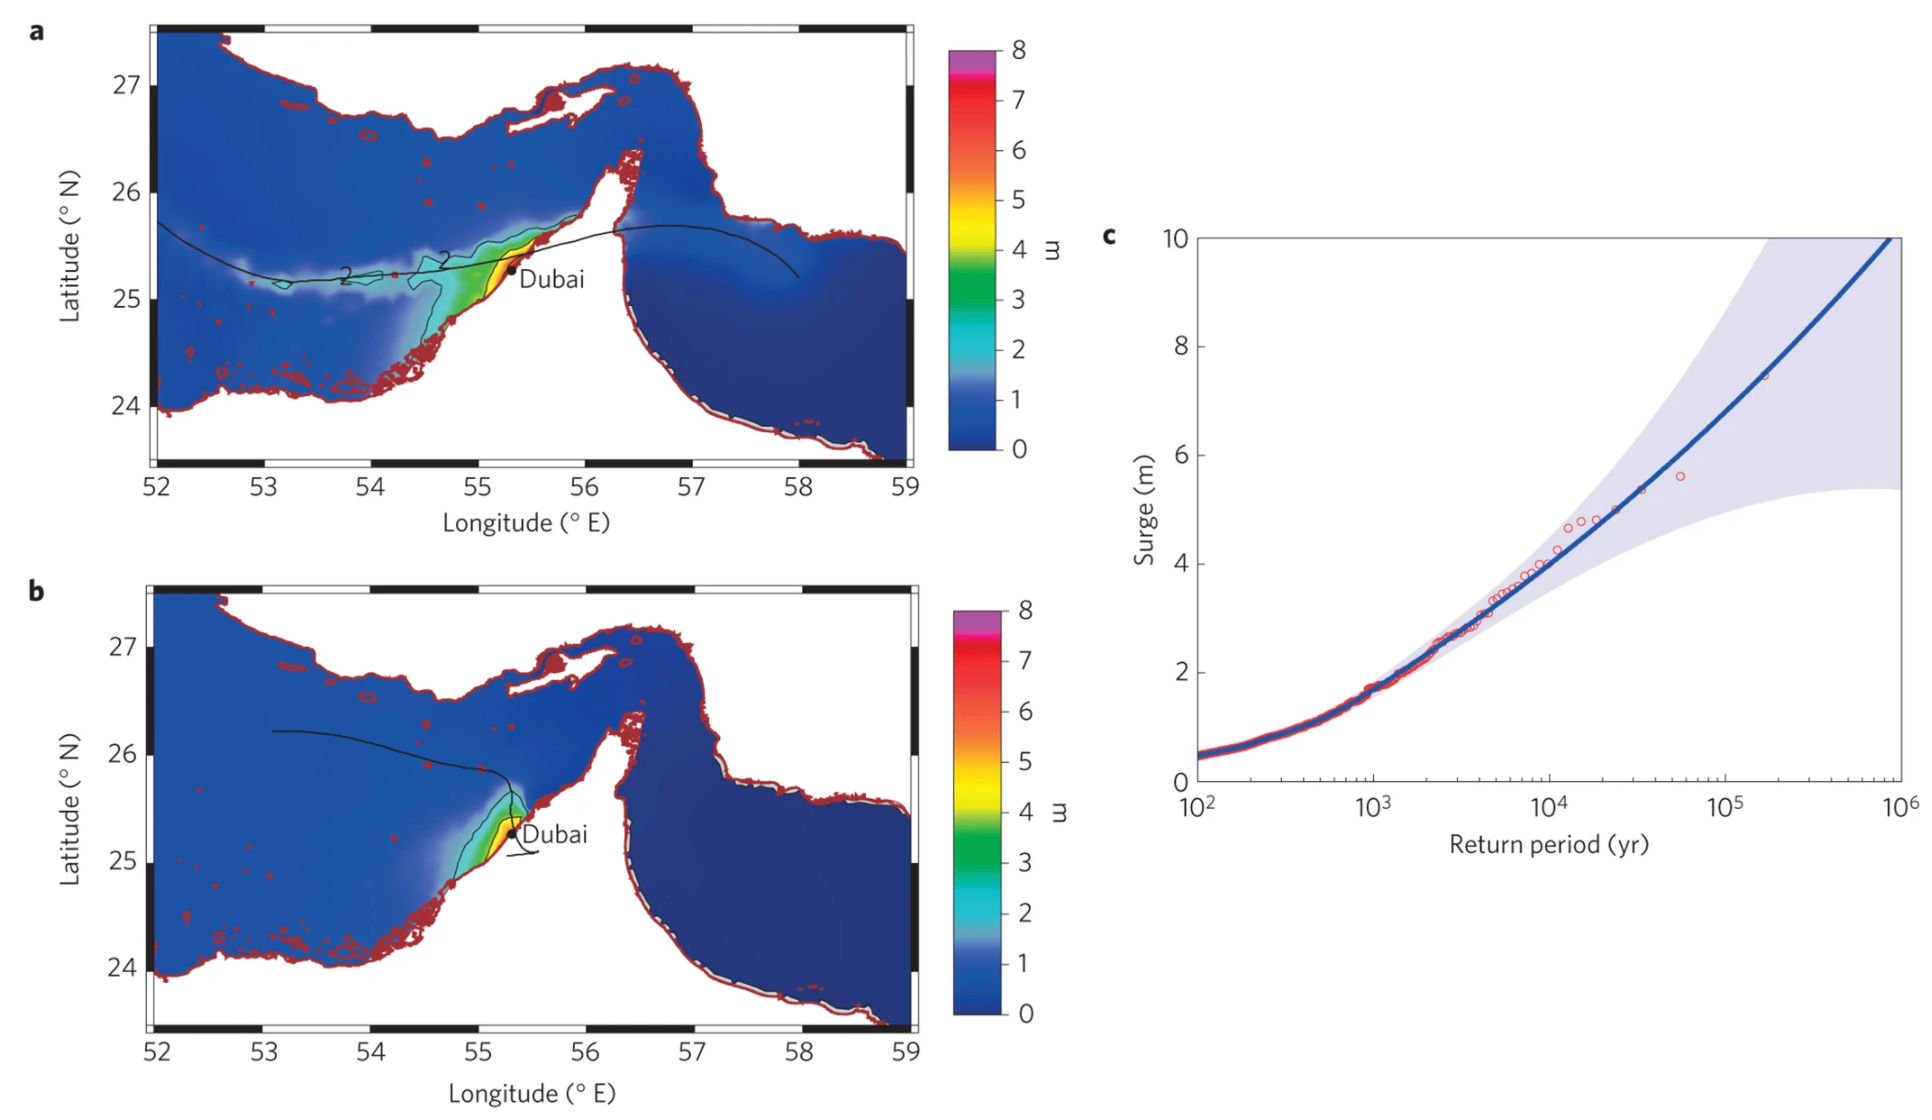
\includegraphics[width=\linewidth]{dubai.png}
    \caption{Figure 5 from~\cite{Lin2015GreyCyclones}.
            (a) and (b) show two of the largest Tropical Cyclones 
            from the physical model with their trajectory
            as a black line, and the maximum height of the 
            storm surge during the event at each point
            on the sea surface as the color map.
            It is very unlikely for a tropical cyclone to hit Dubai,
            but the very warm seas around Dubai are able 
            to sustain very intense tropical cyclones.
            Panel (c) shows a return period vs.~return 
            level plot for the coastal point at Dubai.
            The fit line is convex at every point, 
            indicating it is a member of the Frech\'et class~\cite{coles2001introduction}, so that 
            it has no finite upper bound.
            }
    \label{fig:DUBAI-FRECHET}

\end{figure}


\begin{itemize}
    \item The tropical cyclone is a heat engine running between the 
          sea surface and the tropopause. Therefore, by the second law of
          thermodynamics its maximum efficiency of `potential intensity'
          is given by the efficiency of a Carnot engine running between
          the two heat reservoirs~\cite{emanuel1986air, emanuel1987dependence}
          (see Figure~\ref{fig:carnot}).
    
    \item Assuming that the temperatures of the sea surface
          and tropopause are bounded, this also implies that
          the potential intensity is bounded.
    
    \item Given that the maximum height of a storm surge is
          a product of the response function and the surge, 
          where the response function is bounded, then the
          maximum height of the storm surge is bounded.
    
    \item However, in some parts of the literature the storm surge
        is fitted by an unbounded process by a Frech\'et fit (see Figure~\ref{fig:DUBAI-FRECHET}).
        Notably the example given in Figure~\ref{fig:DUBAI-FRECHET}
        is for an area in which the tropical cyclones are very severe,
        and quite unlikely to happen.
        This would make this point the most susceptible to not having 
        enough examples in the model run to accurately
        describe their distribution. Therefore the presence of 
        a Frech\'et distribution might suggest that we are pre-asymptotic.
    
    \item If the extreme value distributions are proven from assuming that
        we are in the limit, then does this not suggest that they would not
        hold in the case that we are pre-asymptotic~\cite{Galambos1978TheStatistics}.
    
    \item Therefore, perhaps every published example of a Frech\'et fit
        is proof that insufficient data was gathered to model the
        extreme value distribution for storm surges.
    
    \item If tropical cyclones are a bounded phenomenon \cite{emanuel1986air}, and extreme value theory is only valid in the asymptotic limit, is every published example of a Frech\'et fit a contradiction? (see e.g. Figure 5 in \cite{Lin2015GreyCyclones}).
    
    \item \cite{Cirillo2020TailDiseases} showed that a spurious Frech\'et fit could be dealt with for pandemics.
    
    
    
\end{itemize}

\section{Publication schedule}
\label{sec:pub}

As scientific work is largely useless unless its results are communicated 
to the wider community, it makes sense to plan work so that it 
falls into work that could coherently be communicated as a paper.
A rough schedule for the work is given in Table~\ref{tab:schedule}.
As research is creative work, strict time horizons, or the feasibility of 
a particular study cannot be guaranteed. Generally, I think the first
couple of papers are a much more `sure thing', and later papers 
are much more speculative.
Each publication should be accompanied with their respective code and 
documentation to ensure that all of the work reaches the 
highest scientific standards for reproducibility and is FAIR.
Roughly 6 months is set aside at the end of the PhD to 
write and refine the c.~200 page final thesis. 
Hopefully earlier peer reviewed publication should provide a strong
basis to do this.

\subsection{Papers}

\begin{enumerate}

    \item MRes work `A Parsimonious Coupled Model of the Equatorial Pacific Surface Temperature Change'.
    \begin{itemize}
        \item Co-authors: Dan Jones (BAS), Naomi Henderson (Lamont), Mark Cane (Lamont)\footnote{Of El Ni\~no predicting fame.}
        \item     I emailed the convener of the AGU2021 session 
        \textit{`A082 - Multi-Scale Processes in the East Pacific
        Intertropical Convergence Zone'} with a summary of my MRes
        work\footnote{\url{https://seager19.readthedocs.io/}} 
        and he encouraged me to submit this to his session, 
        which will provide me with an opportunity to gather feedback
        on what expansion the community thinks would be most beneficial.
        \item         With some expansion and adaptation it should be 
        worth turning this work into a paper of its own.
        The bulk of this work should be done before the PhD 
        begins, and submitted or close to submission before AGU.
        \item Having Mark Cane as a co-author should ensure high standards
            and a relatively simple peer review process.
    \end{itemize}
    
    \item Replicating and expanding upon
        C13~\cite{Chavas2013U.S.Perspective} 
        should take up about 3-6 months at the beginning 
        of the PhD. If the work is a significant enough 
        improvement this should be submitted to a relevant journal
        so that it is some way through the review process 
        by the first year report.
    
    \item Emulating storm surge models using different 
        machine learning models, different physically 
        constrained machine learning models, and simplified
        physical models. The only comparable article I can find
        is~\cite{Ma2020MultifidelitySurge} where the only use
        a Gaussian process. This work is likely to take longer, 
        perhaps 6-9 months. It could form the backbone
        of the first year report, but it is unlikely
        to be published by then.
    
    \item Quantifying the performance of each storm surge replacement
        model on the historical period when forced with ECMWF/ORAS4
        data, in comparison to US East coast tidal gauge. 
        Look at extreme events and baseline conditions. 
        Attempts at correcting for the change in resolution.
    
    \item Further verification of the extreme events reanalysis models 
        ensemble over a larger number of points, potentially expanding to
         instrumented areas of East Asia. This should pick out which
         models generalise the best.
         
    \item If the previous three steps of the verification work, then 
        try to apply this to the the output of a CMIP model
        with a similar structure to the ECMWF reanalysis product.
        If this is successful, 
        then apply it to as many CMIP models as can be justified, 
        and try to produce a rough guess, with uncertainty bars, 
        as to the change in hazard over as many decades as 
        can be justified in the areas for which the models have been 
        well validated.
        
\end{enumerate}

\begin{table}[htb!]
    \centering
    \begin{tabular}{llllllllllllll}
    \hline \hline
    \textbf{Paper} & Q3 & Q4 & Q1 & Q2 & Q3 & Q4 & Q1 
    & Q2 & Q3 & Q4 & Q1 & Q2 & Q3 \\
    \hline
        1 & X   \\
        2 & & X & X \\
        3 & & & X & X & X \\
        4 & & &  &  &  & X & X &\\
        5 & & &  &  &  &  & &  X & X & \\
        6 & & &  &  &  &  & &   &  & X & X &\\
        \hline
        Thesis &&&& &&&& &&&& X & X\\
        \hline \hline
    \end{tabular}
    \caption{Rough schedule for which paper would need 
            to be worked on when in the PhD to submit 
            the PhD thesis in summer 2024. It is possible
            that to make a substantial contribution,
            different papers could be combined, or if the work 
            doesn't work then perhaps pieces of work will end up
            without their own publication.}
    \label{tab:schedule}
\end{table}

\subsection{Programming packages}

Potential standalone pip packages:

\begin{enumerate}
    \item \texttt{seager19}: Seager et al.~19~\cite{seager2019strengthening} model coupled at every time step in pure python.
    \item \texttt{coastlines}:
    Methods for extracting coastlines from climate models using xarray, 
    collecting them into organised coastlines, and calculating metrics.
    Possible metrics include the fractal dimension of the coast,
    the convexity, roughness, bathymetric properties, etc.
\end{enumerate}

\section{Supervision Arrangements}

Dr.~Daniel~C.~Jones (British Antarctic Survey) has agreed to be my primary
supervisor. Dan Jones has a broad background in computational mathematics and 
environmental physics, which should allow Dan to provide good advice.
We have been having weekly hourly meetings, although this schedule could
change depending on whatever is helpful.

Dr.~Michael Herzog (Department of Geography) is primarily involved with 
the physical numerical modelling of tropospheric processes, and is
knowledgeable about broader scale global processes.
Dr.~John Taylor (Department of Applied Mathematics and Theoretical Physics)
is a much more theoretically/analytically motivated scientist,
with special knowledge about submesoscale ocean processes.
I expect him to have more interest in idealised and simplified
models for the storm surge.
Their involvement will probably depend on how much they are 
interested in each subproject.

Prof.~Dan Chavas (Purdue) and Prof.~Talea Mayo (Emory) might
be drawn into collaborative work,
but this work will all be unofficial and outside of university structures.
Prof.~Dan Chavas is an expert on the physics of tropical cyclones, and in 
particular their size. Prof.~Talea Mayo is an expert on storm surge models,
extreme value theory, and advanced methods of data assimilation.

Prof.~Laure Zanna (NYU) was involved in the project at the MSci stage, and she could
become involved again if she expresses interest.

\end{document}
